\chapter{The DCC Subsystem}

The LCS core library builds the software foundation for implementing the layout control software. So far we have discussed the general working, node and port functions and callbacks. One part that was only touched upon briefly so far is the digital command control \texttt{(DCC)} subsystem. A significant part of the LCS messages deal with the control of running equipment decoder, stationary decoders and the track itself.

This chapter now dives a little deeper into the DCC subsystem. At the heart of this subsystem is the base station node that is in charge for of managing locomotives and tracks. It receives LCS messages from devices such as a cab throttle and translates these commands into a series of DCC packets. The packets are the basis for the DCC track power modules to actually produce the electrical signals on the track. The power module is either a part of the base station or a separate booster. Base station, boosters and throttles are just nodes making use of the DCC commands in the LCS message set. They too can implement reacting to events and send themselves events. First we will look at a base station and what it takes to manage a locomotive session and to generate the DCC packets for mobile and stationary decoders. Next, we will look into how a DCC packet actually gets out on the track.

\section{Locomotive session management}

Digital locomotives are equipped with a mobile decoder. The decoder will analyze the DCC packets on the track and if addressed perform the desired function. For each active locomotive the base station first establishes a locomotive session. Across the layout, a locomotive is uniquely identified by its **cabId**. In DCC terms this is the address of the locomotive. The DCC standard defines an address range that all decoders, mobile and stationary, share. Once a session is established for the cabId, the base station accepts LCS DCC commands, such as setting the speed, direction or a function, and produce the corresponding DCC packet. We will see later what happens to the packet.

A base station typically works with two DCC tracks. There is the **main track**, which consist of all the track sections of the layout. Commands such as setting a locomotive speed and direction, refer to this track. In addition, there is a **service track** which is used to configure an individual locomotive. This track is electrically separated from the main track. However, when it comes to packet transmission, the two tracks are very similar. For the base station functionality there are thus two key functional components. The first is the locomotive session management, the second is the programming of a locomotive mobile decoder. The programming track commands do not need a cabId, i.e. address, as there should only be one locomotive on this track. This has to do with the way a decoder replies the base station and will be discussed when we talk about decoder programming.

\section{Stationary Decoders}

While mobile decoders can be found in a locomotive, a stationary decoder can be found somewhere on the layout. For example, a stationary decoder that is close to a set of turnouts. It is connected to the main track and just like its mobile cousin decodes the DCC packets. Stationary decoders, called accessories in the NMRA standard, are assigned to a part of the address range and react to their configured address. The base station accepts LCS commands for such a decoder and generates the DCC packets for it.

As said before, the trend is to use a layout control system with a dedicated bus for the layout components. The key idea is to offload the track where the engines run from the packets for the accessories. Another approach is to have a dedicated wire to all accessory decoders and send the DCC packets on this. In a sense another track without locomotives. Our layout control system will support generating the stationary decoders packets and send them via the main track.  But the feature is only implemented for completeness. Maybe there is still one old decoders that is put to use this way. Our layout will be controlled by the LCS bus.

\section{DCC packet generation}

The key task of the locomotive session management is to generate the DCC packets for running and configuring mobile and stationary decoders. There are also packets, such as RESET or IDLE, that concern all decoders on the track. The DCC packets are described officially in the NMRA specifications. The *RailCommunity* specification documents ( RCN-xxx) also have an excellent description of the packets layout and their interpretation. Each bit is either a zero or a one. A "one" bit has a period of 116 microseconds, a zero bit a period of 232 microseconds. The exact timings are listed on the DCC standard, for now, this is a good enough description. The appendix contains links to their web pages for diving into all the details of the DCC packet format and protocol.

The base station part that produces DCC packets is not concerned with how these packets are actually transmitted to the locomotive. This is the task of the DCC track management component, which will be presented shortly. In general, a DCC packet is a stream of bits consisting of the preamble, a decoder address and the command bytes followed by a checksum byte. The preamble is to sync a decoder with the upcoming data stream. The address tells which decoder is address and the command bytes actually tell what needs to be done. Finally, the checksum makes sure that there was no error in transmitting the packet. The following figure shows a simple packet.

picture 

\begin{figure}[h]
    \centering
   % 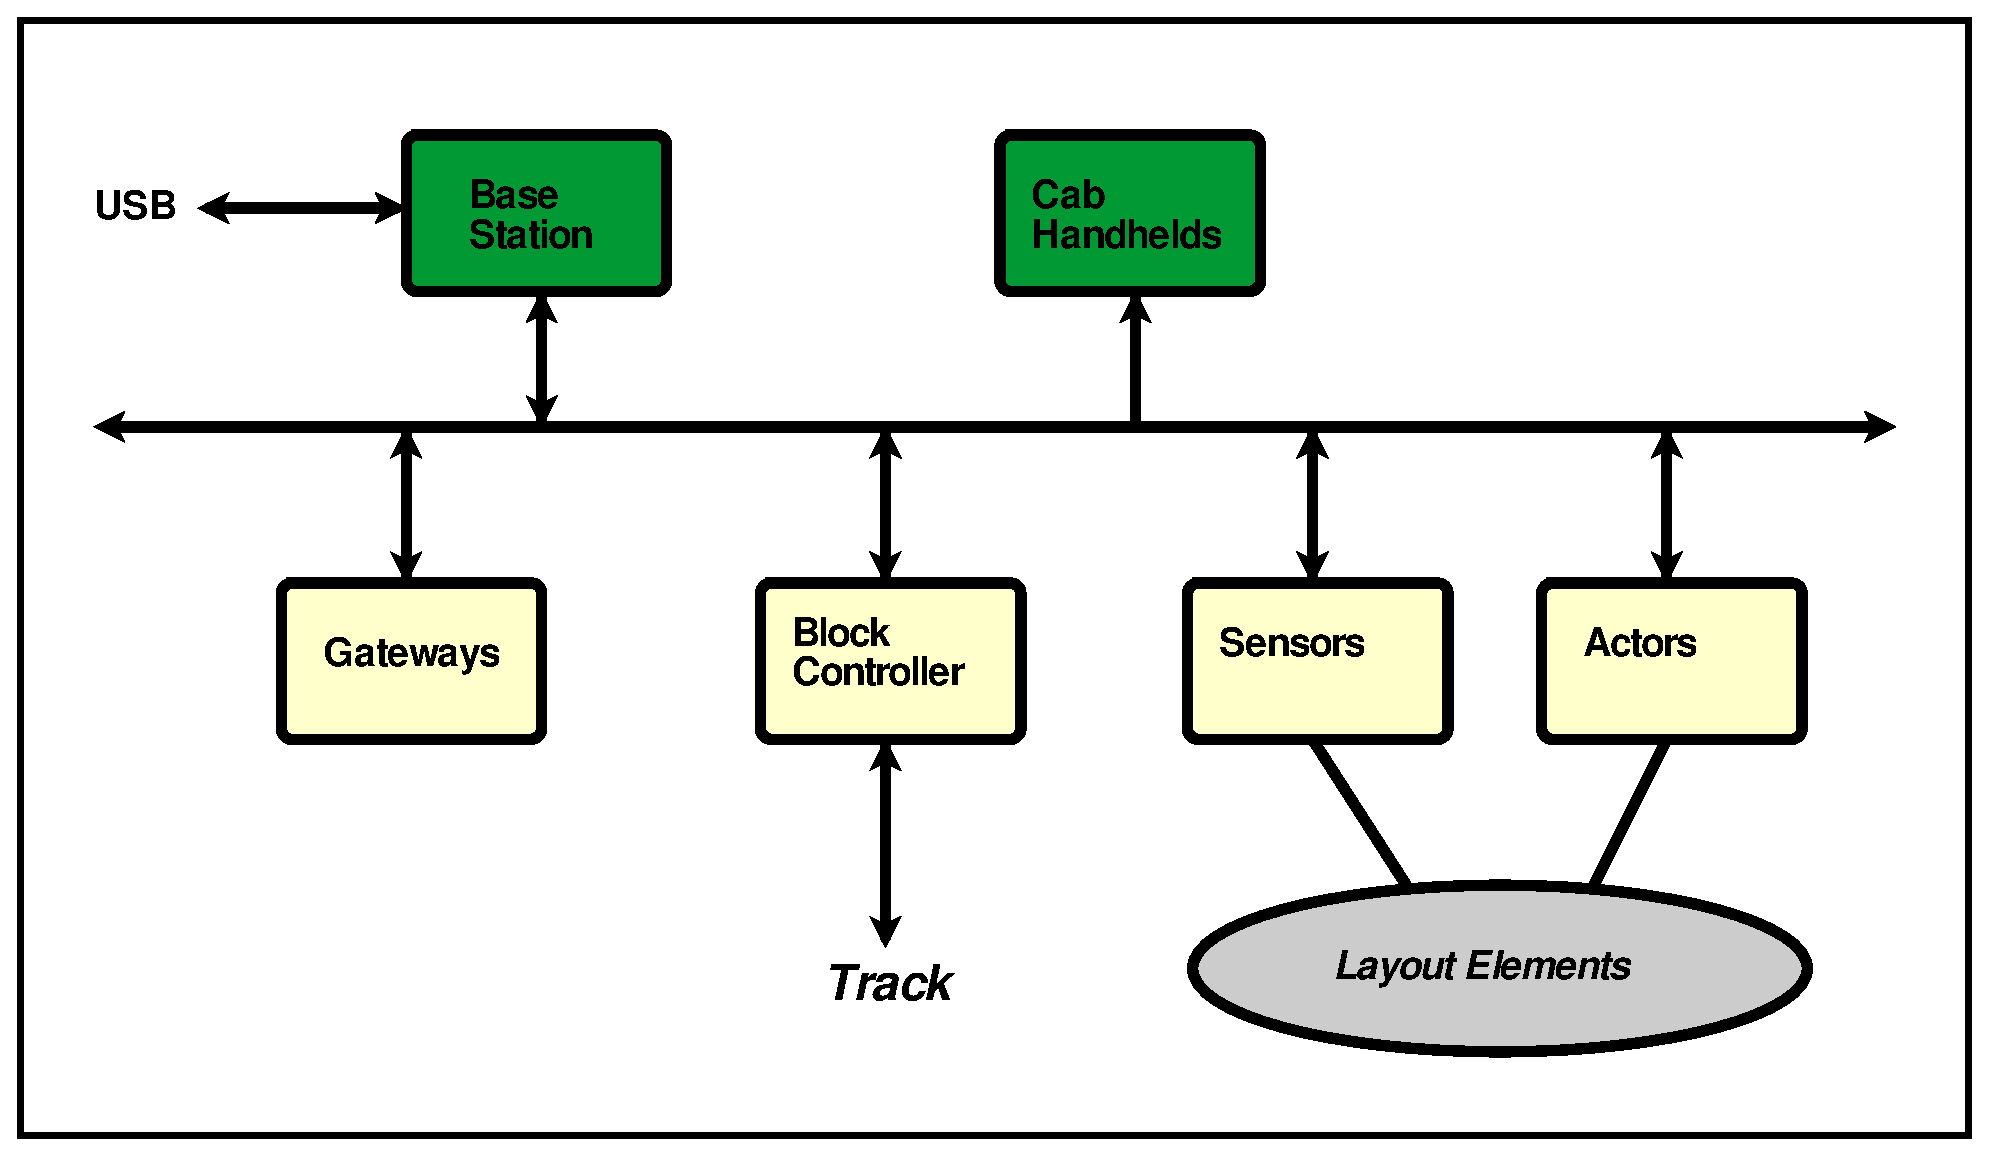
\includegraphics[page=1, width=\textwidth]{./figures/Schematic_LcsNodes-Layout-Overview.pdf}
   %![Schematic_LcsNodes-DCC-Packet-Structure.png](./Figures/Schematic_LcsNodes-DCC-Packet-Structure.png )
\end{figure}

The high level LCS DCC commands are translated by the base station into the corresponding DCC packets. There are two modes of transmission. With the first mode, any incoming command is translated and sent out immediately with an optional repeat count. Consider a locomotive speed stop command. This has of course top priority. The second mode of transmission is a one time fixed sequence of DCC packets for a high level LCS command, such as it is used for programming a decoder.

When no command is pending, the base station will loop through all active session entries and send packets for refreshing the previously sent commands. For example, after sending a speed/direction command, this command will be repeated periodically, until a new command is issued for this locomotive session. While looping through the session table, only a part of the necessary refresh packets are generated to make sure that all engines get a fair share of the track bandwidth in time. The complete refresh of speed/direction and function keys are spread over a couple of loop iterations. The DCC standard makes recommendations what data to send out how often or periodically. Time to discuss how the DCC packets actually get to the track.

\section{Sending a DCC packet}

The DCC track management software component does not store any DCC packets other than the active packet that is currently being transmitted and the pending next packet. If it is busy with sending a packet and there is already a pending packet queued, the packet loading routine in the locomotive session management component is waiting until the pending packet becomes the current packet and then the next packet is queued. There is one more scenario to address. Suppose there is no packet currently sent from the locomotive management and thus there is no packet to send to the track. In this case, we cannot just stop sending packets, as the locomotives draw their track power from the track signal. DCC track management signal generation then just "invents" a packet to send out. This is is the DCC IDLE packet for the main track and the DCC RESET packet for the programming track.

\section{DCC Track Signal Generation}

The primary task of a DCC track signal generator is to receive the DCC packets generated by the base station producing the hardware signals for the packet bits on the track. The other task is to monitor the power consumption and the optional RailCom channel communication. DCC signals are square wave signals with a defined duty cycle period. A duty cycle of 58 microseconds represents a "DCC one", a duty cycle of 116 microseconds a "DCC zero" bit. This signal is sent to the track by reversing the polarity of the two tracks lanes with the respective timing. Typically, a H-Bridge such as found in motor drivers will perform this task. If the H-Bridge is enabled, sending a "DCC One" will mean to set the digital input signals for the H-Bridge to enable the "+" direction, and then reverse the digital signals for the "-" direction. The H-Bridge hardware essentially reverses the track polarity accordingly to digital series and ones. The DCC packet is broken down, bit by bit and the digital signal is produced.  That's it, we have a nice signal on the track. How exactly the base station does the digital signal output generation is discussed in more detail in the base station chapter.

\section{Power consumption monitoring}

DCC track management is also responsible for continuously monitoring the track power consumption. Considering that boosters can emit several Amps a short circuit for a longer time will certainly damage track and running equipment. It is therefore paramount to monitor the actual current consumption very closely. Monitoring track power consumption can be done by measuring the voltage drop over a shunt resistor in serial with the H-Bridge. The controller analog input will periodically read the value and process the incoming data. From a software perspective there are a couple of ways when to measure the voltage and how to process it. One way is to measure at defined spots in the bitstream.

During the signal generation, the track power current consumption will be measured at defined spots in the bit stream. A zero bit in a packet is a good place. The hardware just need to make sure that the measurement completes during the 116us half cycle of the zero bit. But certainly, there are other ways of measuring. When exceeding the configured consumption limit, it is stored in a node variable, DCC track management will broadcast a power overload event and shut down the track. After a configured time a restart is attempted. If the restarting fails for several times, the track is powered down permanently and manual intervention is required.

In addition, care needs to be taken to report a power consumption value that reflects the consumption over a period of time. Most locomotive decoder use a PWM ( pulse width modulation ) approach to drive the motor in the engine. Depending on when the current consumption measurement takes place a high level value or a zero value is returned. This does of course not reflect the actual power consumption. Therefore, several values sampled need to be used to build the "root mean square" value to indicate the actual power consumption.

\section{Decoder programming support}

There it is. A new locomotive unpacked, sitting on the programming track. At a minimum it needs to be told what its locomotive address will be on our layout. This task is accomplished by writing values to the decoder CV variables. A short locomotive address for example is a writing of this address to CV 1.

DCC is a broadcasting protocol. Just like a radio station, you can send but not receive. In order to communicate back the decoder raises its consumption power for specific value and time period to indicate an OK. DCC track management needs to be able to detect this consumption power fluctuation on the programming track. The detection is very similar to the previously discussed power consumption monitoring except that is done in two steps. Before accessing a CV variable, the current decoder power consumption is measured to establish a base line. This base line is then compared with the actual power consumption after the CV access. A fluctuation for the value and time specified by the DCC standard is considered a positive answer.

Reading all CV variables from a sophisticated decoder can easily take several minutes this way. Furthermore this communication will not work on the main track, as there are many locomotives running, making it impossible to detect the raise in power consumption of a single locomotive. There had to be a better way and there is. And there is. It is RailCom.

\section{RailCom support}

RailCom was invented to address the problem of effective back communication on the programming track and also on the main track. DCC track management needs to implemented the basic mechanism for this kind of communication. As the DCC is a broadcasting protocol, no other transmission is possible while it is broadcasting. The key idea of RailCom is to briefly turn off the DCC communication and use this moment of quiescence to transmit back data from the decoder. The period of short circuiting the DCC track is called the cutout period. In addition to to generating the DCC zeroes and ones on the track, DCC track management is also implementing the cutout support.

The following figure depicts the overall signal timing for RailCom support. All the details can be found in the NMRA and RailCommunity standard document including a hardware reference implementation for a RailCom decoder and detector. After the last bit of a packet and during the first bits of the DCC packet preamble, the track signal is turned off, the track is short circuited. The decoder can now send out data to the track and a signal detector can receive that data. The signal is a simple serial signal with a baud rate of 250 Kbits. The following figure shows the overall DCC and RailCom signal timing.

picture 

\begin{figure}[h]
    \centering
   % 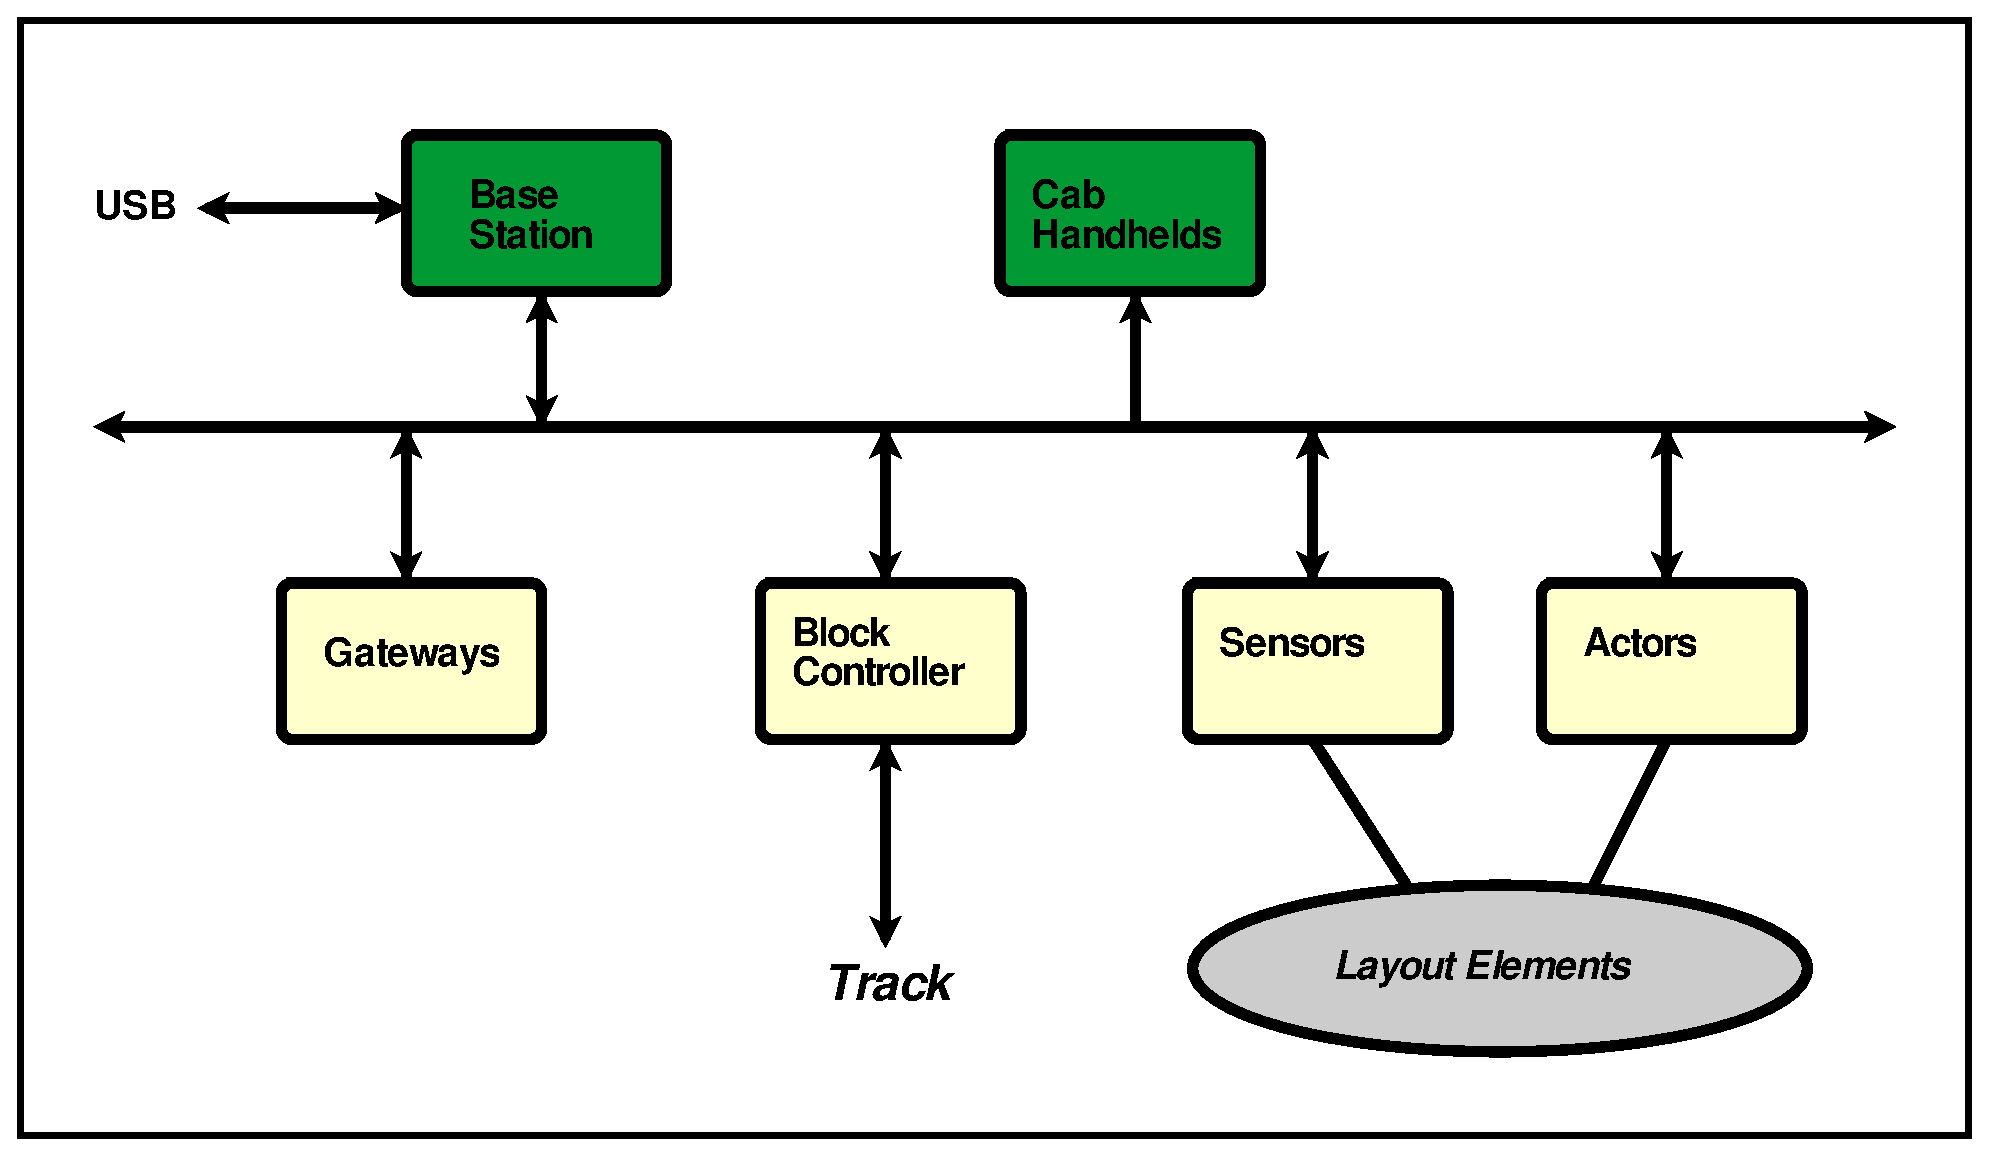
\includegraphics[page=1, width=\textwidth]{./figures/Schematic_LcsNodes-Layout-Overview.pdf}
   %![Schematic_LcsNodes-RailCom-Packet-Structure.png](./Figures/Schematic_LcsNodes-RailCom-Packet-Structure.png )
\end{figure}

The NMRA and RailCommunity standards describe the data format used when sending the RailCom data. There are two channels defined which in total send a maximum 8 bytes during the cutout period. Channel one takes up two bytes, channel two takes up four bytes. To ensure data transmission integrity, the bytes itself are encoded as values with four bits one and four bits zero. This leaves 64 useful values that the byte contains. All else is an invalid data byte. Put together, there are up to 48 bits of data in a RailCom message.

The individual messages available in channel one and two are called datagram. For channel one, a datagram is 12bits, i.e. the six bits encoded in the two raw data bytes, for channel two there are in total 36 bits. Each datagram tarts with a four bit identifier followed by the payload. A decoder is required to transmit its address every time it is addressed on channel one. Decoders will send data on channel two only of explicitly requested. This leaves channel one with a bit of chaos more than one decoder transmits. There are options to tell the decoder to stop sending its ID after an initial couple of times.

Channel two is only used when the decoder is explicitly addressed via an POM or XPOM DCC packet. Still, the base station needs to ensure that multiple requests form different encoders are transmitted one at a time and there is enough tie for the addressed decoder to answer. Als, the decoder needs to be addressed at least twice to complete a data request via RailCom. The first DCC packet tells what to get, the second DCC packet gives the controller a chance to put the RailCom reply in the next cutout packet. Finally, the DCC-A \texttt{(RCN218)} standard uses the RailCom infrastructure for automatic locomotive registration and fast access to the information in the decoder. For this purpose, channel one and two are combined to a 48bits payload data. More on these topics in the base station chapter.

\section{DCC Track sections}

A base station may have a powerful main track and a less powerful programming track. For smaller layouts this is a typical scenario. In fact, the DCC standard requires for the programming track to limit the maximum current to 100mA after initialization to avoid any decoder damage from misconfiguration when testing a new hardware. Larger layouts however are typically divided into several sections each of which is controlled by a DCC booster. This has the key benefit that a short circuit will only affect a track section. A DCC booster can also be equipped with a RailCom detector to implement for example locomotive detection on a per section basis.

To the DCC track management in a base station a booster managing a track section is largely transparent. All track management is concerned with is that the DCC signals are generated. A base station for a larger layout could just have two H-Bridges with a low current rating. One would produce the DCC signal for the main track, the other for the programming track. The programming track output is directly connected to the programming track. The main track output of the base station however is just a signal line that is then fed via the LCS bus data lines into the booster. All track sections will receive the same DCC signal. All boosters are required to be wired with the same track polarity.

picture 

\begin{figure}[h]
    \centering
   % 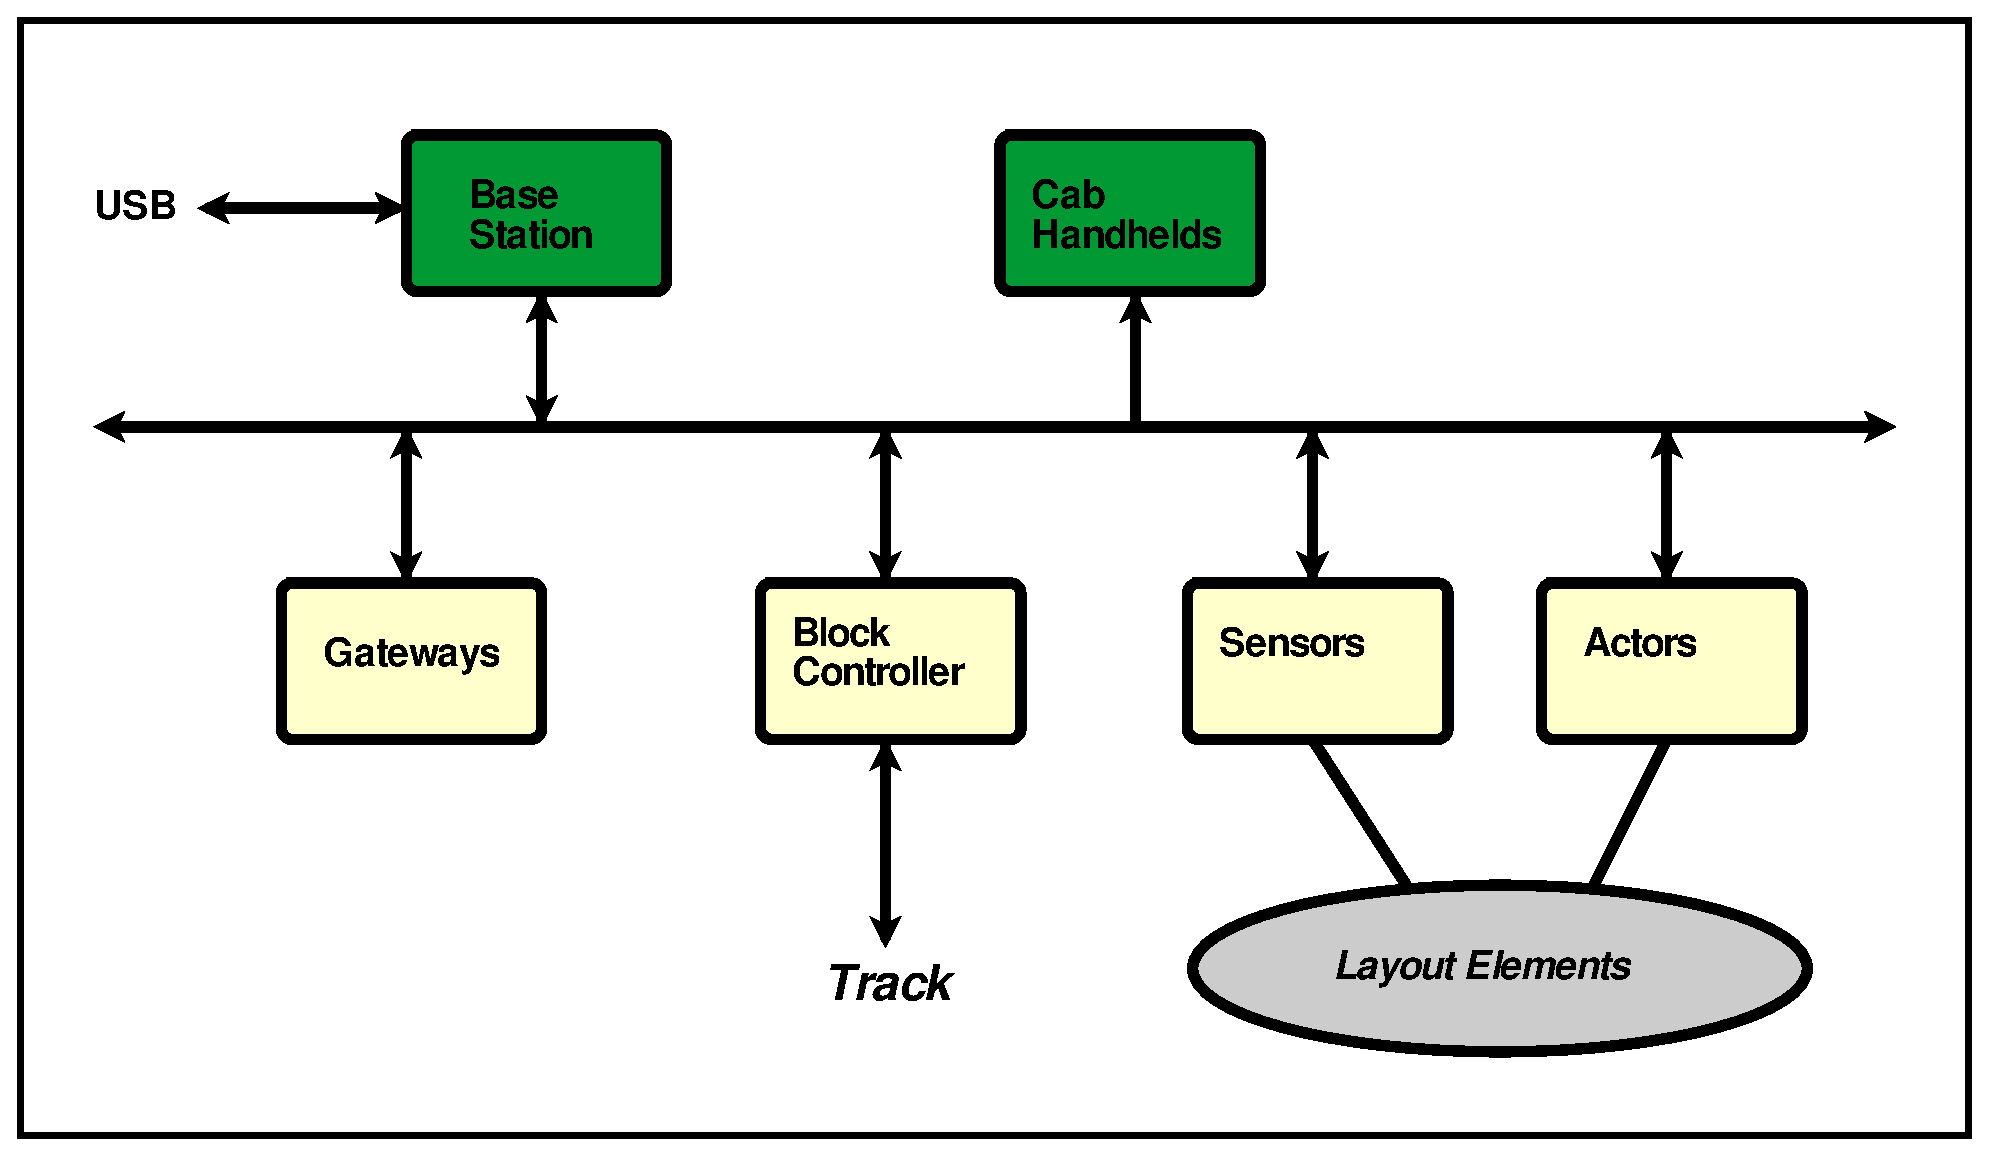
\includegraphics[page=1, width=\textwidth]{./figures/Schematic_LcsNodes-Layout-Overview.pdf}
   %![Schematic_LcsNodes-DCC-Track-Sections.png](./Figures/Schematic_LcsNodes-DCC-Track-Sections.png )
\end{figure}

All boosters will measure the power consumption continuously and in the case of exceeding the limits, send an event that the base station is interested in. Boosters are just LCS nodes like anything else. Port variables and events are the mechanism of communication. The actual implementation of a booster with variables and events are described in the hardware module chapter on boosters.

There is one more thing to take care of. If a layout consists of more than one track section there is the situation that the two boosters are not in close sync with respect to polarity and signal generation timing. Again, it is first of all very important that all boosters have a common polarity wiring. If not, short circuits caused by running equipment crossing from one section to the other are likely to happen. If RailCom is enabled, the cutout period acts as a short circuit of one section as well. If one booster section is in cutout mode and the adjacent booster not yet, crossing rolling equipment would effectively short circuit the active booster. To avoid this problem, boosters need not only be in close sync, the also should feature a kind of "security gap" period before starting the cutout period. In this period the booster is put into disconnected mode. This topic is also discussed a bit more in the booster hardware part.

\section{A short Glimpse at Software Implementation}

The DCC base station plays the key role in the DCC subsystem. In addition to manage the locomotive sessions and generating the necessary DCC packets, it is also responsible to manage the two tracks MAIN and PROG. Built on top of the LCS library, the base station will have two key software components, one for session management and one for track management. The session management part is rather straightforward, a table of active locomotive sessions that are processed periodically. The track management part is by nature very close to the hardware. Two interlinked state machines, one for track signal generation and one for track power management build the core of tack management. The actual implementation of the two key parts of the base station module is described in more detail in the base station chapter.

\section{Summary}

This chapter gave a high level overview on the DCC subsystem. The base station and booster firmware implement the DCC decoder management and track signal generation. Locomotive session management is concerned with managing the running equipment. The key concept is the session, which contains all data needed to control a locomotive on the track. DCC Packets for all active locomotives are generated and sent to the track management component and thereafter periodically refreshed. Programming a locomotive decoder sends a DCC packet sequence which the decoder addressed interprets. There are two tracks, the main track and the programming track. While they are a different in what they are used for and what hardware capacities they need, both will just as their key function putting out the packets generated by the locomotive session management software.

DCC track management is responsible for the track signal generation and track power management. It takes the DCC packets and sends them out bit by bit. First the preamble and optional cutout period then each data byte of the packet. The track consumption power is monitored for the main tack and also used for the programming track decoder acknowledge power consumption fluctuation. Exceeding the configured power consumption limits will result an a shutdown of the signal followed by a number of restarts. The DCC signals produced by the based station are ready to be used and can directly be fed to a track. However, in larger layouts, there will track sections with a DCC boosters for each section. Base station and boosters are, you guessed it, just nodes on the LCS Bus.
